\chapter{Interrupts}
\label{chp:int}
\index{Interrupts}
\label{lbl:int}

\section{Introduction}
Interrupts are mechanisms by which the user code interrupts the execution of the processor and passes control to the kernel to accomplish low level functionalities like disk access, arithmetic exception handling etc.

\textbf{Interrupt Service Routine(ISR)} : The kernel provides routines to accomplish the functionality for which an interrupt has been generated. These routines are known as Interrupt Service Routines. \index{Interrupts!Interrupt Service Routine}

\textbf{Note: } Every ISR should end with an IRET instruction.

\section{The \texttt{INT} instruction}
\label{interrupts}
The instruction used to generate an interrupt is \texttt{INT}. \\ Syntax : \texttt{INT} \emph{n} 

The INT instruction passes control to the Interrupt Service Routine (ISR) for this interrupt located at the physical address 
computed using the value n.

Address computation is done as follows. 
The physical address of the ISR corresponding to interrupt number $n$ is given by:
\begin{equation*} 
\mbox{Physical Address} = (56+n) \times \mbox{Page Size}
\end{equation*}

\index{Interrupts!Table}
Figure~\ref{interrupt table} summarises the physical address to which the control is transferred for each interrupt. Note that the interrupts are disabled once this instruction is executed, since we do not allow interrupts to occur in kernel mode.

\begin{figure}[htp!]
	\centering
	\renewcommand{\arraystretch}{1.2}
	\begin{tabular}{cccc}
		\toprule
		Interrupt No. & \multicolumn{3}{c}{Word Address} \\ \cline{2-4}
		& Page No. & Offset & Address \\ \midrule
		0 & 56       & 0      & $56\times256+0$=$14336$ \\
		1 & 57       & 0      & $57\times256+0$=$14592$ \\
		2 & 58       & 0      & $58\times256+0$=$14848$ \\
		3 & 59       & 0      & $59\times256+0$=$15104$ \\
		4 & 60       & 0      & $60\times256+0$=$15360$ \\
		5 & 61       & 0      & $61\times256+0$=$15616$ \\
		6 & 62       & 0      & $62\times256+0$=$15872$ \\
		7 & 63       & 0      & $63\times256+0$=$16128$ \\
		\bottomrule
	\end{tabular}
	\caption{Interrupts and their locations in the memory}
	\label{interrupt table}
\end{figure}

\memoryLayout{fig:main memory8}

\section{Types of Interrupts}
\index{Interrupts!Types}
There are 8 interrupts (numbered from 0 to 7) supported by the {\ESIM} architecture. The interrupts 0 is a hardware interrupts and the remaining interrupts (1 to 7) are software interrupts.\\

Details of the \emph{hardware interrupt} is as follows.

\begin{itemize}
	\item \texttt{INT 0 :} This is the timer interrupt \index{Timer} which interrupts the processor forcing a context switch. It contains the code for the scheduler of the operating system (refer section~\ref{chp:scheduler}), which schedules the CPU time among the various active processes. Note that this interrupt is machine generated and cannot be called.
%	\item \texttt{INT 7 :} It is generated when the following exceptions\footnote{An exception is an abnormal condition that arises when the machine deviates from its normal execution pattern.} occur:
%	\begin{enumerate}
%		\item \emph{Illegal memory access :} occurs when any address generated by the process does not
%		lie in the range [0, 959].
%		\item \emph{Arithmetic exception :} occurs when divisor is 0.
%		\item \emph{Illegal instruction :} occurs when an attempt is made to execute an instruction not belonging to the instruction set and also when the operands to the instruction is not legal. Eg: \texttt{MOV 4 R0}, \texttt{MOV IP 4} when executed in user mode. These instructions are considered illegal.
%		\item \emph{Stack overflow and stack underflow :} Stack overflow occurs when the value in the SPregister exceeds 959 and stack underflow occurs when the value falls below 768.
%	\end{enumerate}
\end{itemize}
%Refer chapter~\ref{chp:exception} for to know more about the way exceptions are handled.

Details of \emph{software interrupts} are as follows.
\begin{itemize}
	\item \texttt{INT 1--4:} These interrupts are used for the various file system calls. (Refer section~\ref{fssyscall} for File System Calls)
	\item \texttt{INT 5--7:} These interrupts are used for the various process system calls. (Refer section~\ref{procsyscall} for Process System Calls)
\end{itemize}
The interrupts 1--7  are unprivileged and can be called from user mode.

% TODO Should explain how interrupts are serviced ? i,e. give some assembly code ? Probably can be given in appendix.

\section{Calling Convention}
\label{callconv}
\index{Calling Convention}
In this section, we explain the calling and returning conventions for interrupts.\footnote{The convention given above is already built into the AP-SIL compiler. It has been given only to help you understand the internal workings better.}

\subsection{Calling Convention}
Before switching the control to the ISR using the INT instruction the user program does the following:
\begin{enumerate}
	\item Push a dummy value for storing the return value of the interrupt onto the stack.
	\item Push the arguments to the interrupt.
	\item Make the Interrupt call using the INT instruction.
\end{enumerate}

The INT instruction pushes the IP+1 value on to the stack and then starts the execution of the corresponding ISR. When the ISR finishes its execution, IRET instruction is called. This IRET instruction pops the IP+1 value from the stack top into the IP register and the execution of the user program is resumed from the point where it was interrupted.

\subsection{Returning Convention}
After returning from the ISR using the IRET instruction the user program does the following:
\begin{enumerate}
	\item Pop out the arguments from the stack.
	\item Pop out the return value.
\end{enumerate}

Figure~\ref{fig:calling_convention} explains the state of the stack at various stages.

\begin{figure}[htp!]
	\centering
	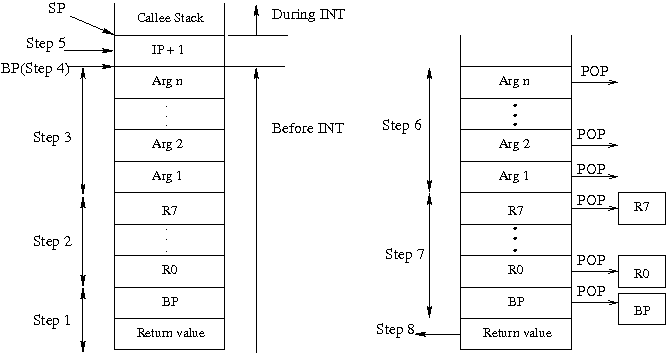
\includegraphics[scale=0.55]{pics/calling_convention}
	\caption{Recommended calling and returning convention for interrupts}
	\label{fig:calling_convention}
\end{figure}
